\documentclass{article}
\usepackage[utf8]{inputenc}
\usepackage{amsthm}
\usepackage{amsmath}
\newtheoremstyle{mystyle}% name
  {\topsep}% Space above
  {\topsep}% Space below
  {\normalfont}% Body font
  {}% Indent amount
  {\bfseries}% Theorem head font
  {}%Punctuation after theorem head
  {.5em}%Space after theorem head
  {}% theorem head spec
\theoremstyle{mystyle}
\newtheorem{prob}{Problem}
\usepackage{graphicx}
\usepackage{wrapfig}
 %preamble
\title{EN.520.216 Homework 4}
\author{LJ Gonzales}
\date{March 2023}

\begin{document}
\maketitle
\begin{prob}
	\begin{enumerate}
	\item
	\end{enumerate}
\end{prob}

\begin{prob}
	\begin{enumerate}
	\item $V_d = V_{dd}-I_{ds}R_1$ where $I_{ds}=\frac{k'W}{2L}(V_{gs}-V_T)^2(1+\lambda V_{ds})$, assuming saturation mode.
We have $V_{gs}=V_g-V_s=\frac{10K*V_{dd}}{20K}-(I_{ds}*1K)=0.9-1000I_{ds}$, and $V_{ds}=V_d-V_s= V_{dd}-2000I_{ds}-(1000I_{ds})=1.8-3000I_{ds}$.
		We then have $I_{ds}=\frac{171}{2}(0.9-1000I_{ds}-0.5)^2(1+0.09(1.8-3000I_{ds}))$.

		Solving graphically, this third degree polynomial has three solutions: at $x\approx397.9\mu A, x\approx402.1\mu A ,x\approx4303\mu A$.
	
	The latter one would imply that the output voltage $V_d$ is $ -6.806V$, which is outside the available swing.
	On the other hand, using $x=397.9\mu A$ and $402.1\mu A$ gives $1.0042$ and $ 0.9958$V, respectively, both of which seem possible. \\
	To confirm whether the assumption of saturation was correct, we need to verify $V_{d} \geq V_{g}-V_T$.
	We have $V_g-V_T=0.9-0.5=0.4$: the inequality is satisfied for both remaining cases.
\item $V_G =\frac{10KVdd}{10K+10K}= 0.9V$.
\item $V_S = 1000I_{DS}= 0.3979V$, using the first potential value of $I_{ds}$ as found previously.
\item We let $I_{D}=397.4\mu A$, albeit with little justification over the other. 
\item $g_m=\frac{dI_{ds}}{dV_{gs}}=\frac{2I_d}{V_{gs}-V_T}$ in simplified form. This is $\frac{2*397.9\mu}{0.9-0.3979-0.5} \approx378.952$mA/V.
\item $r_o=\frac{dId_s}{dV_{ds}}=\frac{d}{dV_{ds}}\frac{k'W}{2L}(V_{gs}-V_t)^2(1+\lambda V_{ds})=\frac{\lambda I_d}{1+\lambda V_{ds}} =\frac{0.09*397.4\mu}{1+0.09*(1.0042-0.3979)}= 33.92\mu A/V$.
	\end{enumerate}
\end{prob}

\begin{prob}
	\begin{enumerate}
	\item In a transistor model where we can't ignore body effects, we have $V_T=V_{To}+\gamma(\sqrt{-V_{bs}+2\phi}-\sqrt{2\phi})$.
	This can be derived from the expression defining the parameters that contribute to the creation of the n channel.
	We have forced our transistor to ground, so $V_{bs}=-V_s$ or, $V_s=-2\phi + (\frac{V_t-V_{to}}{\gamma}+\sqrt{2\phi})^2$
	, from which we know $2\phi=0.9$, $V_t-V_{to}=0.2$.
	This gives us $V_s = 1.04V$

\item If the current element shown is a current source, it cannot create a voltage at the gate on its own: the relationship is one-way only.
	If it is an am\emph{meter}, however, we can first assume saturation and solve $100\mu=\frac{k'W}{2L}(V_g-1.04-0.7)^2$ from the saturation equation with no lambda.
	Plugging in our knowns, $V_g = 1.74+\sqrt{\frac{100\mu *2}{171\mu}}$. We do not have a -(square root) possibility since we assume $V_{gs}>V_t$.
	We then have $V_g = 2.82V$. This is consistent with the assumption $V_d \geq V_g-V_T$, where the LHS is 3, and the RHS 2.12
\item With little changes to the above, we have $V_g=1.74+\sqrt{\frac{100\mu*2*2}{171\mu}} = 3.27V$.
	This is still consistent with the saturation assumption since the RHS is still  $0.43V$ below the LHS.
	\end{enumerate}
\end{prob}

\begin{prob}
	\begin{enumerate}
	\item The layout view defines the physical spacial placement of layers to be created by the manufacturing process.
	The extraction automatically associates the schematic nets to the layout nets, which is necessary to simulate the behavior of the layout.
	
\item The DRC makes sure that no foundry design rules (min spacing and size of layers) are violated in the layout draft.
	The LVS takes the final layout iteration and makes sure that all the components in the schematic match the ones created in the layout. Typically, you would run the LVS once the DRC already checks out.

\item The extracted and schematic simulation outputs might be the same, if the designer created a similar geometry than the default one used by the library. 
	However there might be small differences in its behavior (i.e in switching speed if we make the transistor width very wide, for example).

\item
	\begin{enumerate}
		\item \begin{figure}[h]
			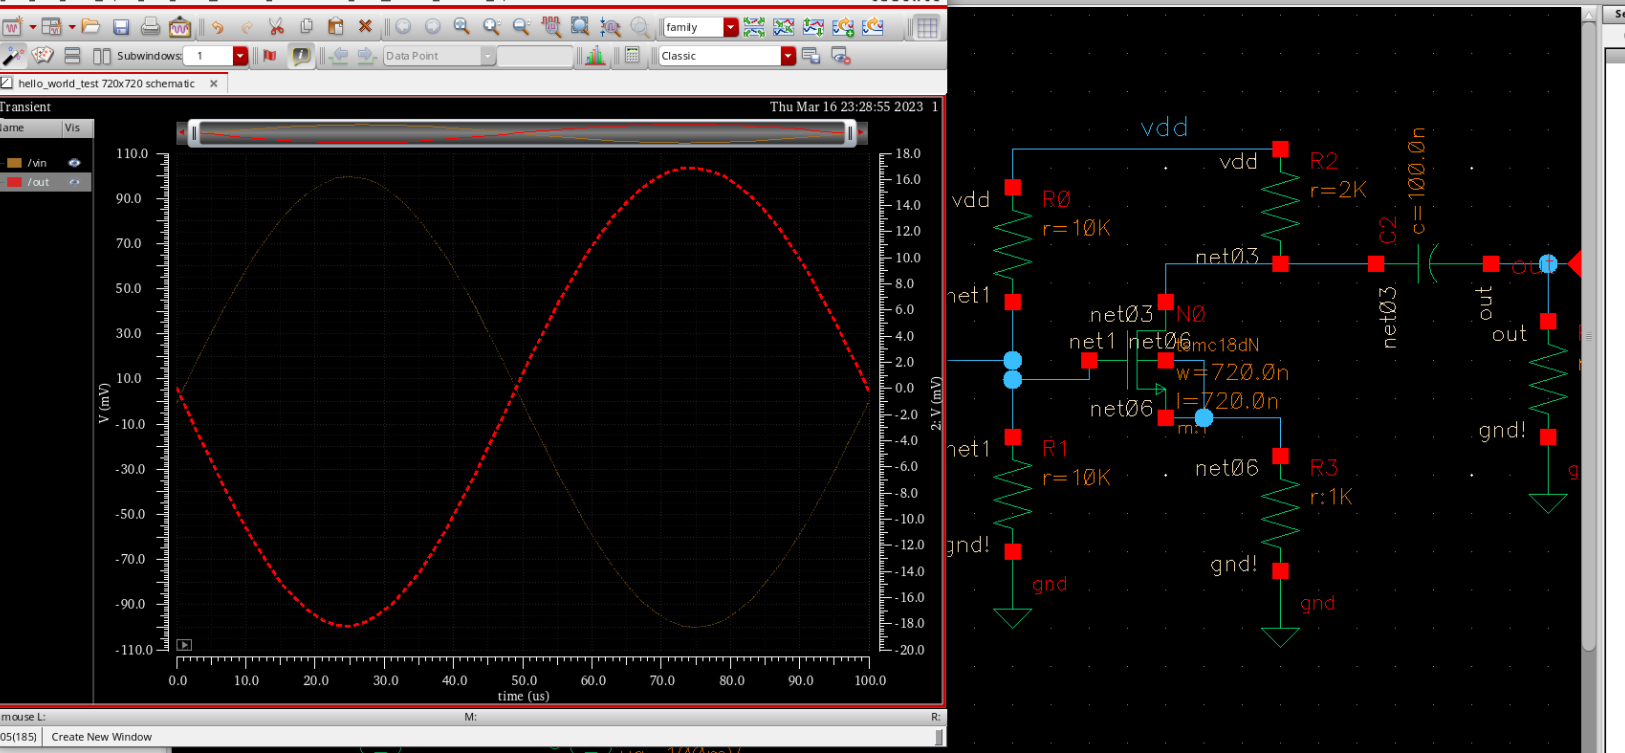
\includegraphics[width =\textwidth]{hw4 files/p1transanalysis.png}
			\label{transanal}
			\caption{Transient analysis with sinusoidal input (separate y axes)}
		\end{figure}
	The input has amplitude 100mV, and the output 17mV and 180degrees out of phase, so $A=-0.17$.	
\item
	\begin{figure}[h]
		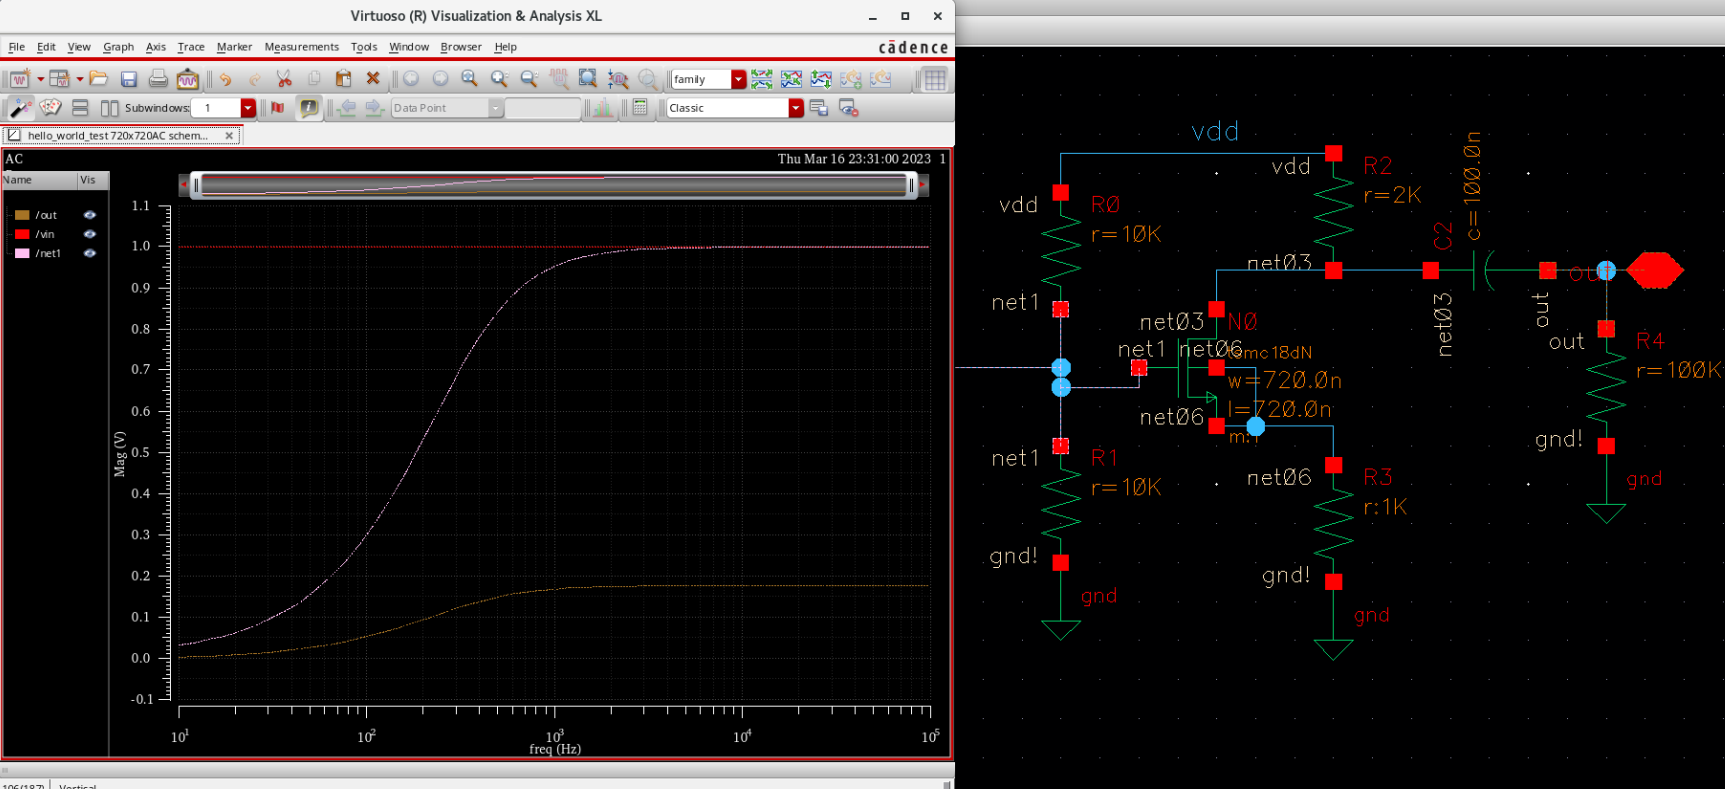
\includegraphics[width =\textwidth]{hw4 files/acanalysis3.png}
		\label{acanal}
		\caption{AC Analysis (output shown on separate axis)}
	\end{figure}
The pole seen at the output is primarily the result of the voltage divider at the input, $R1||R2$ in series with the frequency-dependent load $Z_{C1}$. 
\item Vin is constant throughout the sweep, which makes sense because it is the controlled voltage (amplitude 100mV)
	As for Vg, it matches Vin only when the frequency is high enough that the capacitor acts as a short: in lower frequency regimes, it approaches 0 as $R1||R2 << Z_{cap}$.
	Vo is then a replica of $Vg$ scaled by the absolute value of the gain, $\approx0.17$.
	\end{enumerate}
	\end{enumerate}
\end{prob}

\end{document}
